\documentclass[12pt]{article}

\usepackage{styles/log-style}

\begin{document}
\begin{titlepage}
\begin{center}
\bfseries

{\Large Московский Авиационный Институт\\ (национальный исследовательский университет)}

\vspace{36pt}

\large Институт информационных технологий и прикладной математики

\vspace{36pt}

\large Кафедра вычислительной математики и программирования

\vspace{48pt}

Журнал по исследовательской практике (индивидуальный план)

\end{center}

\vspace{120pt}

\begin{flushleft}
\begin{tabular}{|r|l|}
\hline
Студенты & Группа \\
\hline
Тарпанов Даниил Александрович & М8О-307Б-19 \\
\hline
Ежов Никита Павлович & М8О-307Б-19 \\
\hline
Полюбин Арсений Игоревич & М8О-306Б-19 \\
\hline
Команда: & MAI \#40 Ezhov, Polubin, Tarpanov \\
\hline
\end{tabular}
\end{flushleft}

\vspace*{\fill}

\begin{center}
\bfseries
Москва, \the\year
\end{center}
\end{titlepage}

\pagebreak

\subsection*{Сводная таблица за осень \the\year}
\resizebox{\columnwidth}{!}{
\begin{tabular}{|c|c|c|c|c|c|}
\hline
Дата & Название & Время & Место проведения & Решенные задачи & Дорешанные задачи \\
\hline
12.09.2021 & Grand Prix of Dolgoprudny & 11:00-16:00 & Дистанционно & L, O & M\\
\hline
19.09.2021 & Grand Prix of IMO & 11:00-16:00 & Дистанционно & M, O, P, Q & -\\
\hline
26.09.2021 & Grand Prix of XiAn & 11:00-16:00 & Дистанционно & L, N, P & -\\
\hline
10.10.2021 & XXII Открытая Всесибирская олимпиада & 10:00-15:00 & Дистанционно & A & -\\
\hline
24.10.2021 & Grand Prix of Korea & 11:00-16:00 & Дистанционно & A, C, I, K & -\\
\hline
07.11.2021 & Grand Prix of Siberia & 11:00-16:00 & Дистанционно & 3, 8, 13, 14 & -\\
\hline
14.11.2021 & Grand Prix of EDG & 11:00-16:00 & Дистанционно & A, M, N & -\\
\hline
28.11.2021 & Grand Prix of Southern Europe & 11:00-16:00 & Дистанционно & O, P & -\\
\hline
05.12.2021 & Grand Prix of Poland & 11:00-16:00 & Дистанционно & H, N, O, P, R & -\\
\hline
12.12.2021 & Grand Prix of Nanjing & 11:00-16:00 & Дистанционно & A, N, O, Q & -\\
\hline
19.12.2021 & Moscow Regional Contest & 11:00-16:00 & Дистанционно & A, F, N & -\\
\hline
\end{tabular}
}

\subsection*{Явка на контесты}
\resizebox{\columnwidth}{!}{
\begin{tabular}{|c|c|c|}
\hline
Дата & Название & Присутствующие \\
\hline
12.09.2021 & Grand Prix of Dolgoprudny & Ежов, Полюбин, Тарпанов \\
\hline
19.09.2021 & Grand Prix of IMO & Ежов, Полюбин, Тарпанов \\
\hline
26.09.2021 & Grand Prix of XiAn & Ежов, Полюбин, Тарпанов \\
\hline
10.10.2021 & XXII Открытая Всесибирская олимпиада & Ежов, Полюбин, Тарпанов \\
\hline
24.10.2021 & Grand Prix of Korea & Ежов, Полюбин, Тарпанов \\
\hline
07.11.2021 & Grand Prix of Siberia & Ежов, Полюбин, Тарпанов \\
\hline
14.11.2021 & Grand Prix of EDG & Ежов, Полюбин, Тарпанов \\
\hline
28.11.2021 & Grand Prix of Southern Europe & Ежов, Полюбин, Тарпанов \\
\hline
05.12.2021 & Grand Prix of Poland & Ежов, Полюбин, Тарпанов \\
\hline
12.12.2021 & Grand Prix of Nanjing & Ежов, Полюбин, Тарпанов \\
\hline
19.12.2021 & Moscow Regional Contest & Ежов, Полюбин, Тарпанов \\
\hline
\end{tabular}
}

\pagebreak
\section{Stage 1-B: Grand Prix of Dolgoprudny, Division 2}
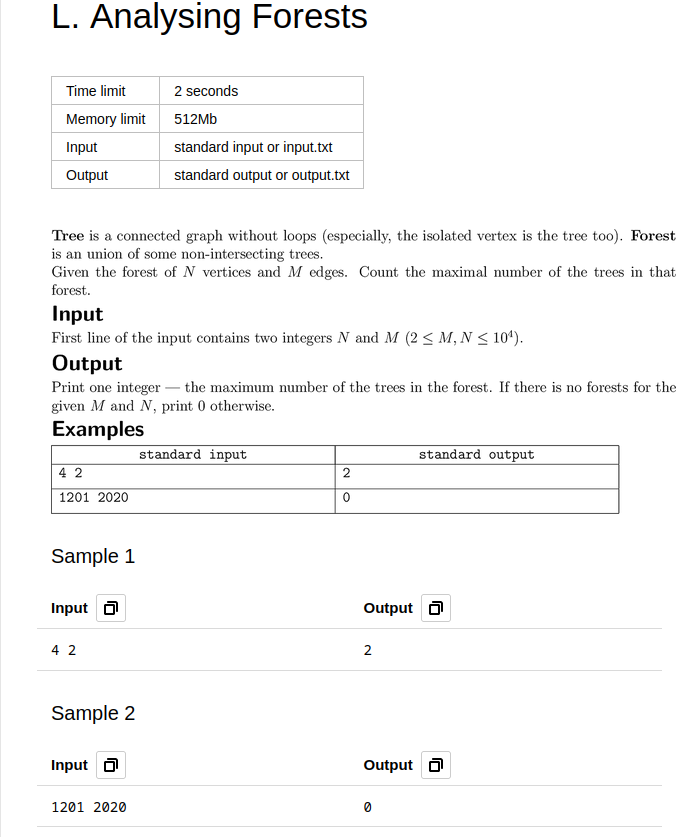
\includegraphics[scale=0.75]{statements/1_L.png}
\subsubsection*{Идея}
Если количество ребёр больше количества вершин, то количество деревьев в графе равно $m-n$,
в ином же случае деревьев в графе нет, а значит их количество равно нулю.
Сложность данного решения - $O(1)$.

\subsubsection*{Исходный код}
\lstinputlisting{src/1_L.cpp}
\subsubsection*{Положение команды}
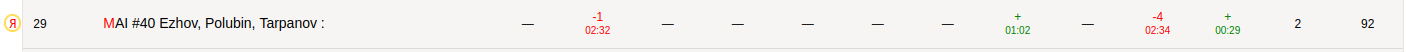
\includegraphics[scale=0.5]{images/1.png}\newline\noindent

\pagebreak
\section{Stage 2-B: Grand Prix of IMO, Division 2}
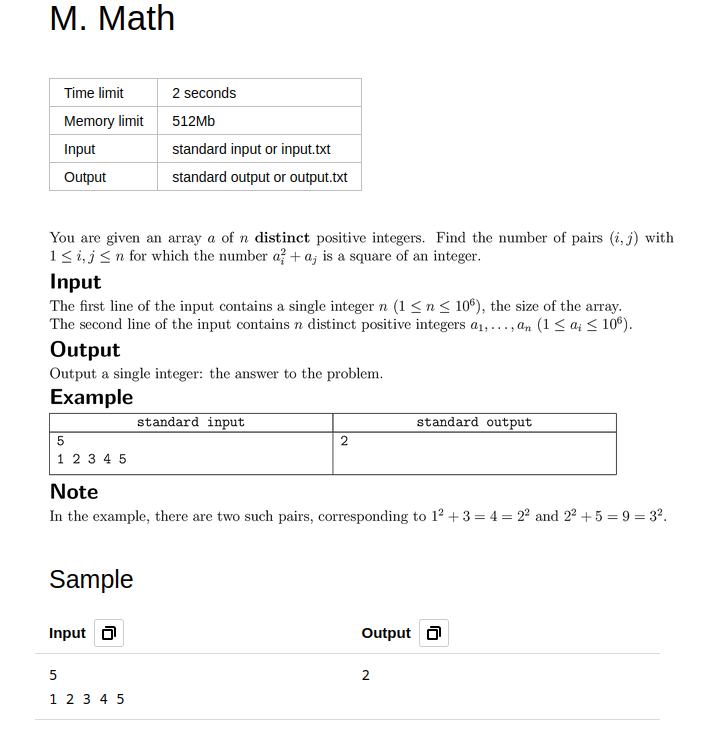
\includegraphics[scale=0.75]{statements/2_M.png}
\subsubsection*{Идея}
Примем $a_i$ как $a$, а $a_j$ как $b$, в таком случае получим, что у нас $a^2 + b = c^2$.
Если мы отсортируем массив исходных чисел, то сможем проверять, существует ли в нашем массиве такое
$b$, котороу удовлетворяет условию, что $b = c^2 + 2 \cdot a \cdot c$ (формула была выведена). Алгоритм заключается в следующем,
после сортировки массива мы начинаем проходить его с начала, перебирая $c$ начиная с 1, пока наш бинарный поиск не начнёт выходить за границы
массива (в таком случае останавливаем while, и переходим к следующему элементу массива). 
\\ 
Сложность данного алгоритма $O(n \cdot k \cdot \log{n})$, где $k$ -
максимальный квадрат, полученный в задаче.
\subsubsection*{Исходный код}
\lstinputlisting{src/2_m.cpp}
\subsubsection*{Положение команды}
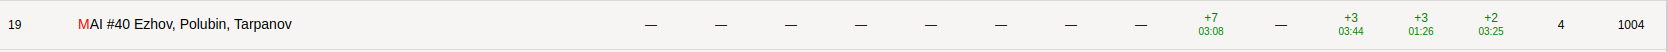
\includegraphics[scale=0.5]{images/2.png}\newline\noindent

\pagebreak
\section{Stage 3-B: Grand Prix of XiAn, Division 2}
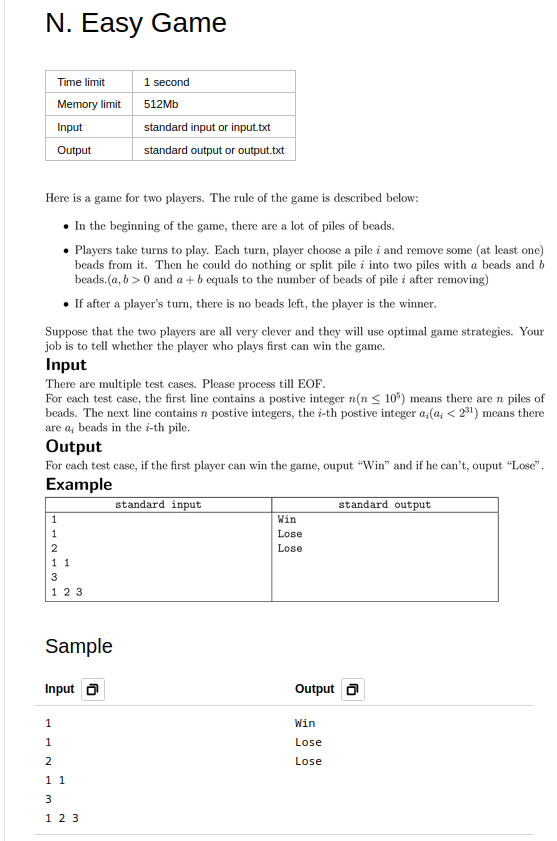
\includegraphics[scale=0.75]{statements/3_N.png}
\subsubsection*{Идея}
Так как в задаче описывается равноправная игра двух игроков, то она 
\\эквивалентна игре "НИМ"\, а это значит, что
для каждых входных данных можно посчитать XOR сумму, если она отлична от нуля, то выигрывает второй игрок, а если нет - первый.
\\ 
Сложность данного алгоритма $O(n \cdot \log{m})$ (чтобы посчитать XOR, нужно $log_2{max(n+m)}$ итераций для чисел $m$ и $n$).
\subsubsection*{Исходный код}
\lstinputlisting{src/3_N.cpp}
\subsubsection*{Положение команды}
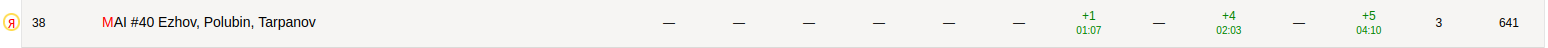
\includegraphics[scale=0.5]{images/3.png}\newline\noindent

\pagebreak
\section{Stage 4-B: Grand Prix of Korea, Division 2}
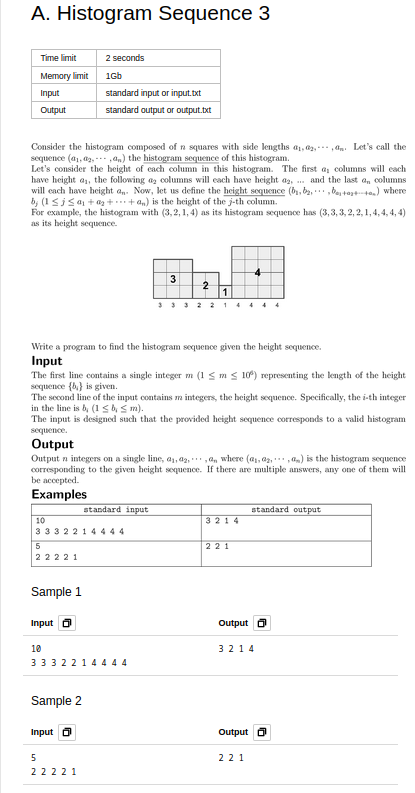
\includegraphics[scale=0.75]{statements/4_A.png}
\subsubsection*{Идея}
Считаем гистограмки....
\\ 
Сложность данного алгоритма $O(n)$
\subsubsection*{Исходный код}
\lstinputlisting{src/4_A.cpp}
\subsubsection*{Положение команды}
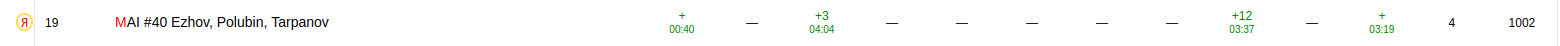
\includegraphics[scale=0.5]{images/4.png}\newline\noindent

\pagebreak
\section{Stage 6-B: Grand Prix of EDG, Div 2}
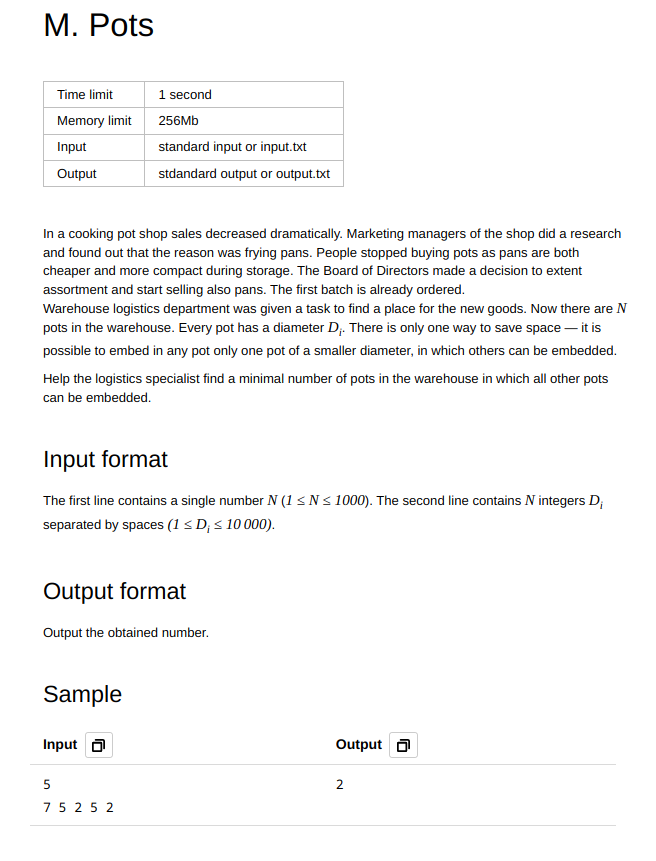
\includegraphics[scale=0.75]{statements/6_M.png}
\subsubsection*{Идея}
Отсортируем все горшки по диаметру. Реализуем функцию, осуществляющую “помещение” наименьшего горшка в первый подходящий по размерам горшок. 
В цикле будем вызывать эту функцию, до момента, пока схлопывание не перестанет происходить.
\\ 
Сложность данного алгоритма $O(n \cdot log{n})$ из-за сортировки
\subsubsection*{Исходный код}
\lstinputlisting{src/6_M.cpp}
\subsubsection*{Положение команды}
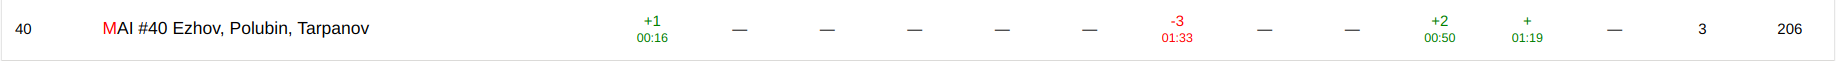
\includegraphics[scale=0.5]{images/6.png}\newline\noindent


\pagebreak
\section{Stage 7-B: Grand Prix of Southeastern Europe, Div 2}
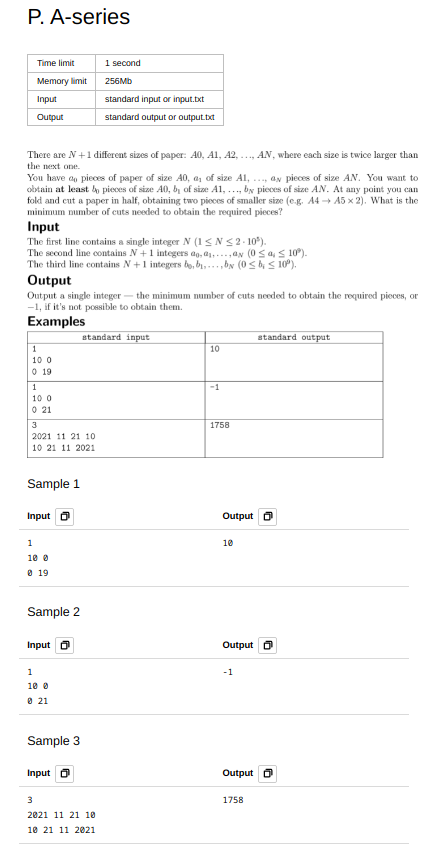
\includegraphics[scale=0.75]{statements/7_P.png}
\subsubsection*{Идея}
Будем итерироваться по двум массивам начиная с конца. На каждой итерации будем вычитать $a[i]$ из $b[i]$. После вычитания, перенесем количество 
листов из $b[i]$ в $b[i-1]$ по следующему принципу: если $b[i] \% 2 == 0$, то перенсем в $b[i-1]$ ровно $b/2$ листов и прибавим к ответу $b[i]/2$. 
В противном случае, перенсем $(b[i] + 1)/2$ листов и прибавим столько же к ответу. В конечном счете, получим новый массив $b$, в  первой ячейке 
которого будет лежать необходимое количество листов размера $A0$. Если $a[0] > b[0]$, то выводится посчитанный ранее ответ, в противном случае 
невозможно порезать листы так, чтобы их хватило.
\\ 
Сложность данного алгоритма $O(n)$
\subsubsection*{Исходный код}
\lstinputlisting{src/7_P.cpp}
\subsubsection*{Положение команды}
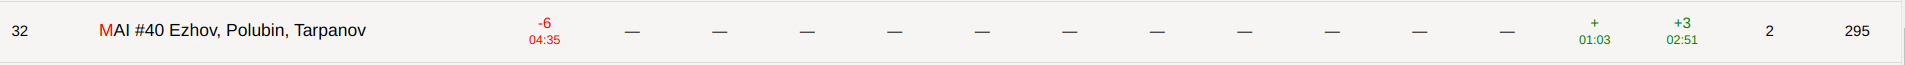
\includegraphics[scale=0.5]{images/7.png}\newline\noindent


\pagebreak
\section{Stage 8-B: Grand Prix of Poland, Div 2}
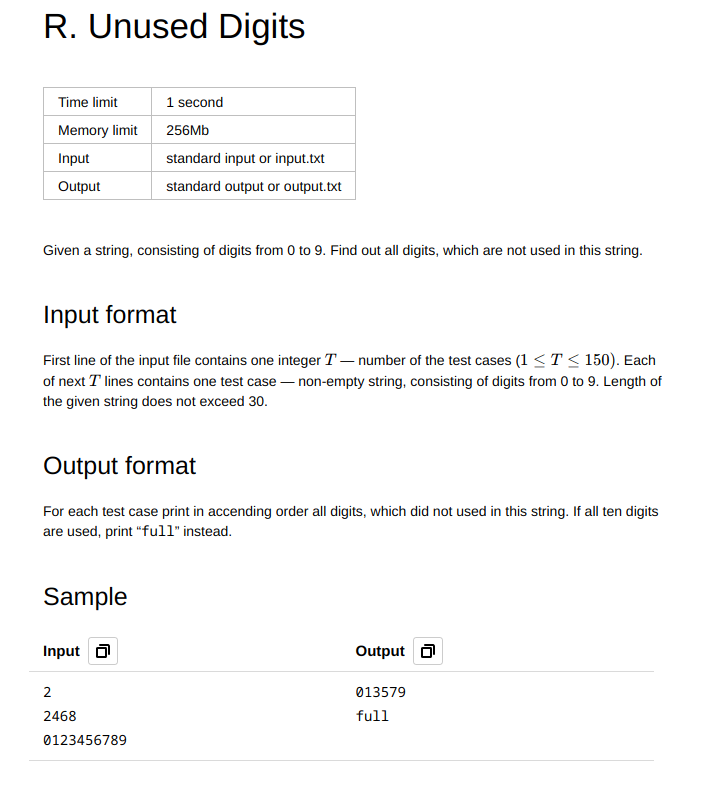
\includegraphics[scale=0.75]{statements/8_R.png}
\subsubsection*{Идея}
Заведем массив used с 10 элементами типа bool, изначально инциализированных как false. Потом пройдемся по строке s и будем присваивать 
$used[s[i] – `0`]$ значение true. После этого на каждое i-oe вхождение true будем добавлять в результирующий массив $i$. Если результирующий 
массив окажется пустым, выведем “full”, иначе выведем все его элементы.
\\ 
Сложность данного алгоритма $O(n)$
\subsubsection*{Исходный код}
\lstinputlisting{src/8_R.cpp}
\subsubsection*{Положение команды}
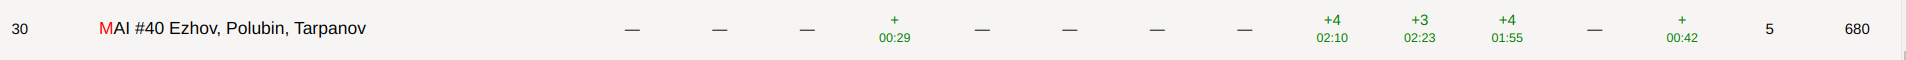
\includegraphics[scale=0.5]{images/8.png}\newline\noindent

\pagebreak
\section{1/4 ICPC}
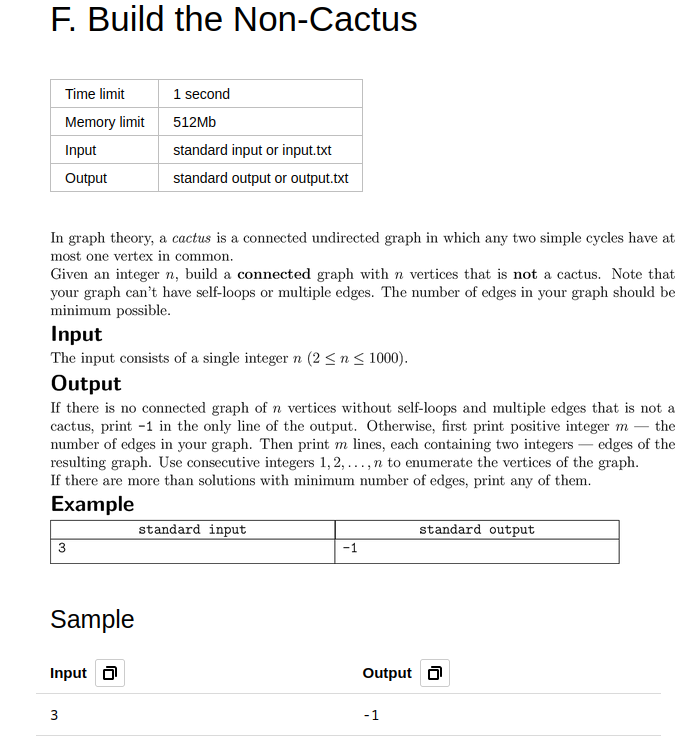
\includegraphics[scale=0.75]{statements/QuarterFinal_F.png}
\subsubsection*{Идея}
Если дано более трех вершин, будем строить “круглый” граф, то есть граф, с ребрами вида [i, i+1], [i+1,i+2]...[i+n, i]. Такое построение 
грантирует минимально возможное количество ребер. После этого, чтобы граф перестал быть кактусом,  нужно провести в нем хорду – ребро между 
двумя несмежными вершинами. Для простоты, в каждом графе соединим вершины 1 и 3.
\\ 
Сложность данного алгоритма $O(n)$
\subsubsection*{Исходный код}
\lstinputlisting{src/QuarterFinal_F.cpp}
\subsubsection*{Положение команды}
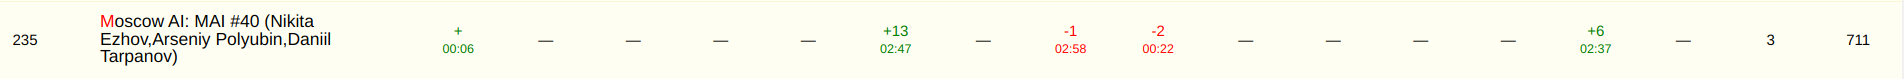
\includegraphics[scale=0.5]{images/QuarterFinal.png}\newline\noindent


\end{document}
